\documentclass{standalone}
\usepackage{tikz}
\tikzset{         block/.style = {draw, fill=white, very thick, rectangle, minimum height=1cm, minimum width=2cm},
}
\begin{document}
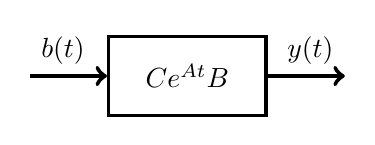
\begin{tikzpicture}[scale=2]
    \node[block](h)at(0,0){$Ce^{At}B$};
    \draw[->,ultra thick](-1,0)node[above right]{$b(t)$}--(h.180);
    \draw[->,ultra thick](h.0)--(1,0)node[above left]{$y(t)$}; 
\end{tikzpicture}
\end{document}